
\documentclass[10pt]{article}

\usepackage{graphicx,amsmath,amssymb,subfigure,enumerate,versions}
\usepackage{multicol,multirow,mdframed}
\usepackage{epstopdf}
\usepackage{pstricks,auto-pst-pdf}
\usepackage{pst-all}
\usepackage{pst-ode}
\usepackage{pst-math}
\usepackage{hyperref}
\usepackage{listings}
%\usepackage{mcode}
\lstset{language=Matlab}
\DeclareGraphicsExtensions{.png,.jpg,.pdf}

% ************ Page Margins *************
\hoffset=-1.3in
\setlength{\textwidth}{7.5in}
%%%%% MARGINS
\topmargin 0pt
\advance \topmargin by -\headheight
\advance \topmargin by -\headsep
\textheight 9.5in

% ************ Shortcuts *************
\newcommand{\Z}{\mbox{\sf Z\hspace{-1.5mm}Z}}
\newcommand{\SolutionSeparator}{ \hfill \hfill \hrule \hfill \hfill }
\newcommand{\R}{\mbox{\rm I\hspace{-0.75mm}R}}
\columnsep=0.75in
\newcommand{\vsc}{\vspace{1mm}}
\newcommand{\D}{\Delta }
\newcommand{\ifd}{f(x)~dx}
\newcommand{\dd}{\frac{dy}{dx} \,} 
\newcommand{\der}[2]{\frac{d{#1}}{d{#2}} \,}
\newcommand{\ddx}[1]{\frac{d {#1}}{dx} \,} 
\newcommand{\ddy}[1]{\frac{d {#1}}{dy} \,} 
\newcommand{\ddz}[1]{\frac{d {#1}}{dz} \,} 
\newcommand{\ddt}[1]{\frac{d {#1}}{dt} \,} 
\newcommand{\ds}{\displaystyle } 
\newcommand{\la}{\lambda } 
\newcommand{\del}{\nabla } 
\newcommand{\zx}{\frac{\partial z}{\partial x} \,}
\newcommand{\zy}{\frac{\partial z}{\partial y} \,}
\newcommand{\dx}{\frac{\partial f}{\partial x} \,}
\newcommand{\dy}{\frac{\partial f}{\partial y} \,}
\newcommand{\pp}[2]{\frac{\partial {#1}}{\partial {#2}} \,}
\newcommand{\ppx}{\frac{\partial }{\partial x} \,}
\newcommand{\ppy}{\frac{\partial }{\partial y} \,}
\renewcommand{\thesection}{\Roman{section}}
\newcommand{\vi}{\vec{i}}
\newcommand{\vj}{\vec{j}}
\newcommand{\vk}{\vec{k}}
\newcommand{\vv}{\vec{v}}
\newcommand{\lan}{\left\langle}
\newcommand{\ran}{\right\rangle}
\newcommand{\degr}{^{\circ}}

% *** Define the printed question style ***
\newcommand{\q}[1]{ {\em #1} }
% \renewcommand{\q}[1]{ {} }

\newcommand{\notice}{ \begin{center}Some problems and solutions
    selected or adapted from \\ Stewart {\em Calculus-Early
      Transcendentals} and Hughes-Hallett {\em Calculus} .\end{center}
}

% *** Overwrite, if desired, the question format
\includeversion{Question} 
\includeversion{Solution}

\newcommand{\multicolstart}{ }
\newcommand{\multicolend}{ }

\renewenvironment{Question}
{ \begin{mdframed}[nobreak=true,hidealllines=true,backgroundcolor=gray!50,innerleftmargin=5ex] }
{ \end{mdframed} }


% *** Footnoting with symbols ***
\long\def\symbolfootnote[#1]#2{\begingroup%
\def\thefootnote{\fnsymbol{footnote}}\footnote[#1]{#2}\endgroup}

\newcommand{\WeekTitleOne}{Derivatives - Foundations}
\newcommand{\WeekTitleTwo}{Derivatives - Linearization and Applications}
\newcommand{\WeekTitleThree}{Derivatives - Modeling}
\newcommand{\WeekTitleFour}{Integrals - Foundations}
\newcommand{\WeekTitleFive}{Integrals - Techniques}
\newcommand{\WeekTitleSix}{Integrals - Modeling}
\newcommand{\WeekTitleSeven}{Differential Equations - }
\newcommand{\WeekTitleEight}{Differential Equations - }
\newcommand{\WeekTitleNine}{Differential Equations - }
\newcommand{\WeekTitleTen}{Linear Algebra - }
\newcommand{\WeekTitleEleven}{Linear Algebra - }
\newcommand{\WeekTitleTwelve}{Linear Algebra - }


\begin{document}

\begin{center}
\subsection*{MNTC P01 - Week \#8 - \WeekTitleEight}
\end{center}

\newcommand{\Fext}{  F_{\mbox{ext}} }
\newcommand{\Fspring}{  F_{\mbox{spring}} }
\newcommand{\Fdamping}{  F_{\mbox{damp}} }

\begin{enumerate}

% ******************************
\item 
  \begin{Question}
    Use \verb@ode45@ to generate a graph of the solution to the
    following DEs, over the specified interval, given the initial
    condition.

\begin{enumerate}
\item $\ds \frac{dy}{dt} = t^2 + y^2$, $y(0) = 0$, and $0 \le t \le 1$.
\item $\ds \frac{dy}{dt} = \sin(t) + \cos(y)$, $y(0) = 0$, and $0 \le t \le 10$.
\item $\ds \frac{dy}{dt} = (1-y^2) + 0.2 \sin(t)$, $y(0) = 0$, and $0 \le t \le 20$.
\end{enumerate}
\end{Question}

\begin{Solution}
Link to the MATLAB code: \\
\href{http://www.mast.queensu.ca/~apsc171/MNTCP01/PracticeProblems/MATLAB/W08DE01.m}{W08DE01.m}

Here are the graphs of the solutions.

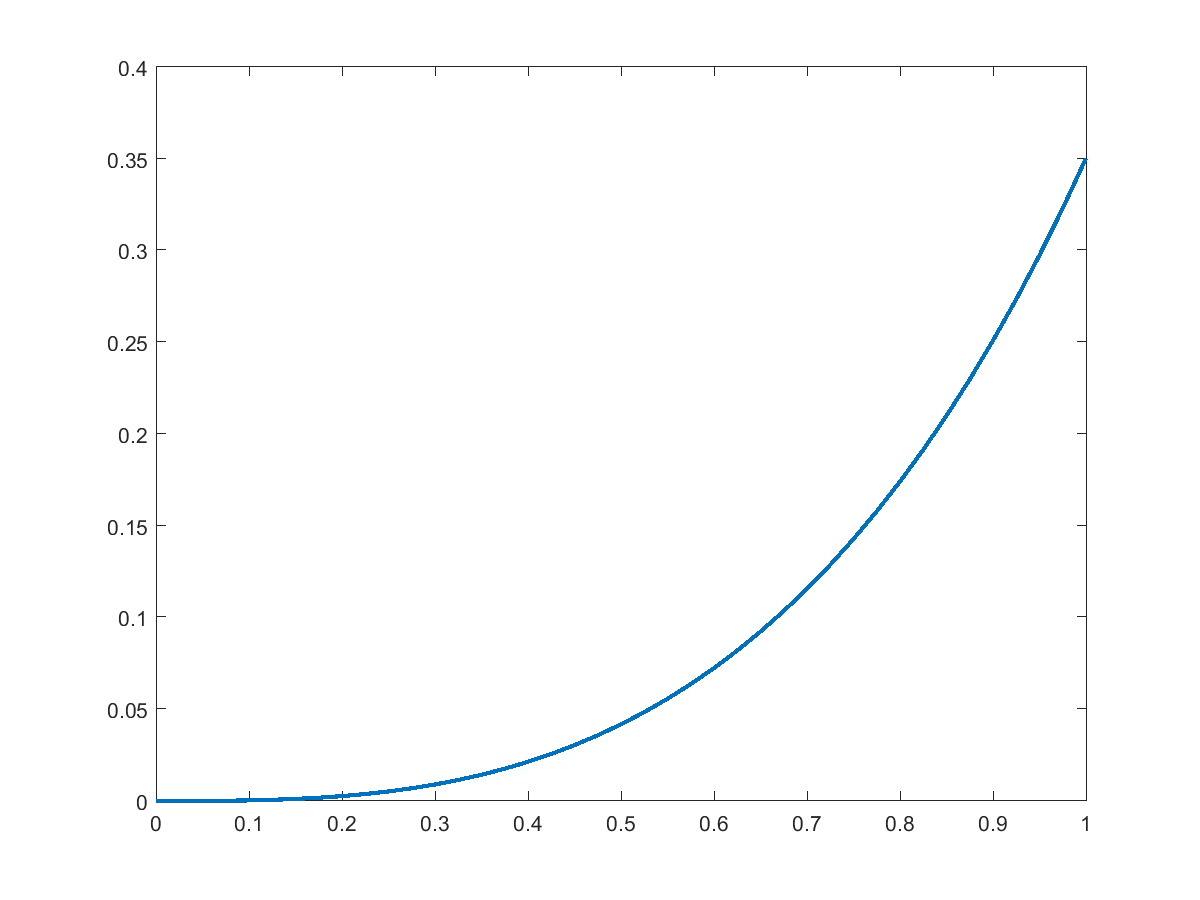
\includegraphics[width = 0.3\linewidth]{graphics/Week08_DESolutions/W08DE01_a} 
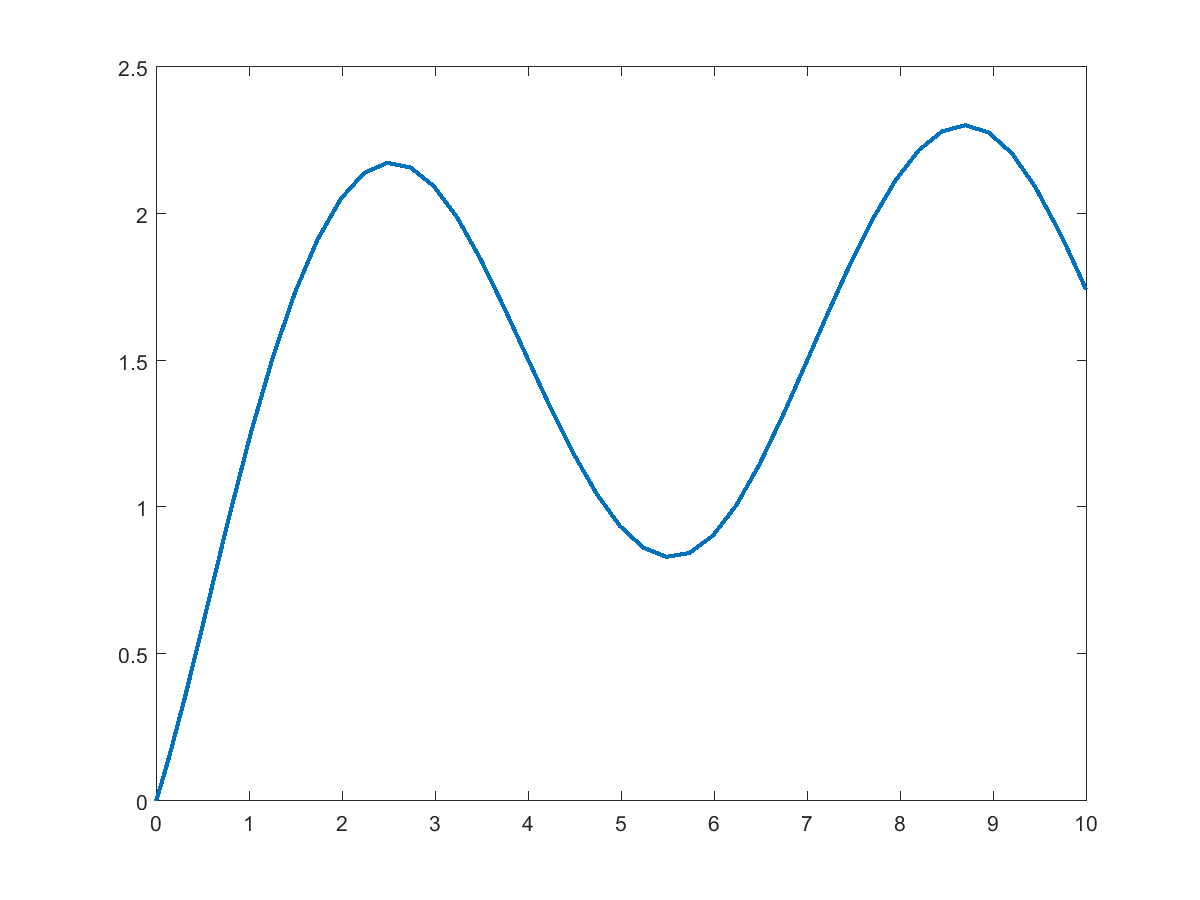
\includegraphics[width = 0.3\linewidth]{graphics/Week08_DESolutions/W08DE01_b} 
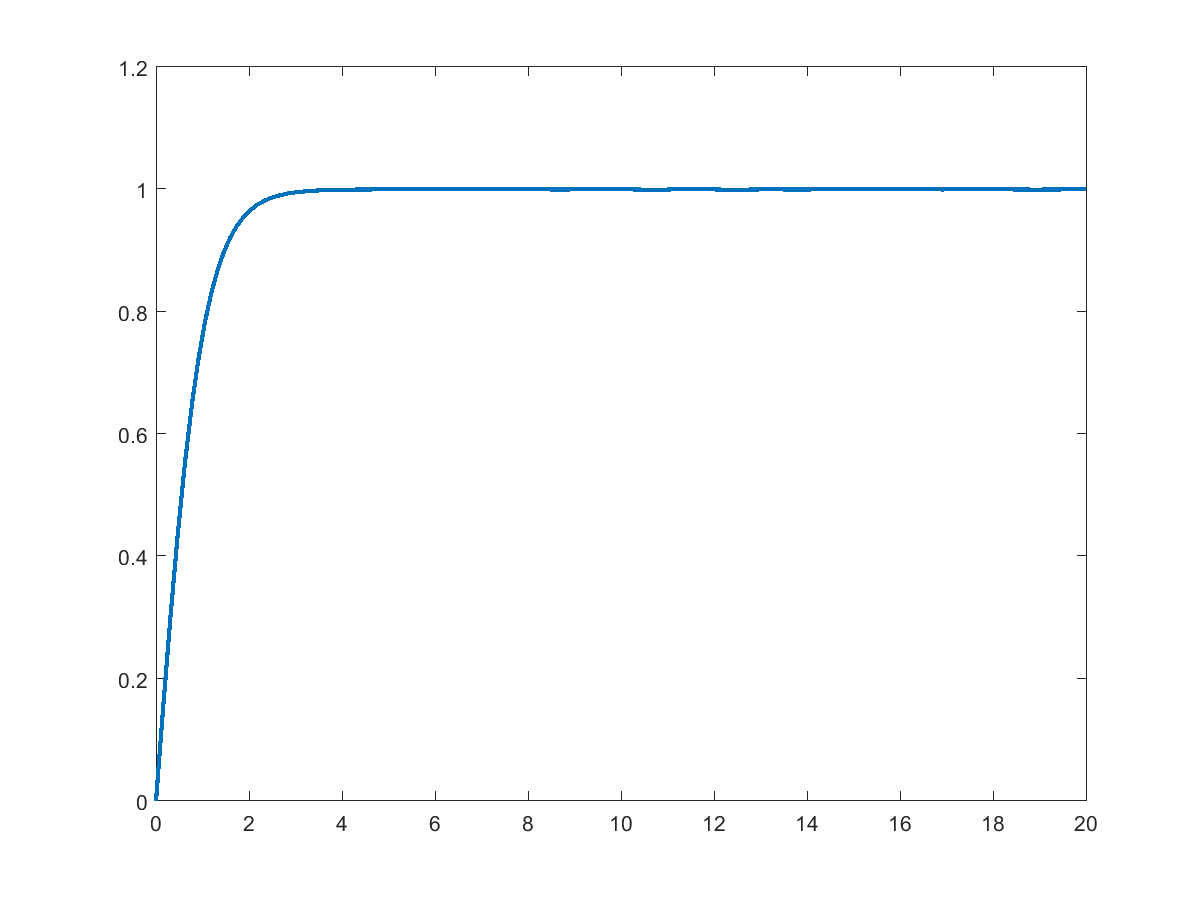
\includegraphics[width = 0.3\linewidth]{graphics/Week08_DESolutions/W08DE01_c} 

\end{Solution} 

% ******************** Newton's Cooling  ********************************
\item 
\begin{Question}
Newton's law of heating and cooling states that an object with
  temperature $T$ in an environment at temperature $T_{ext}$ will heat
  up or cool down according to the differential equation

 $$\frac{dT}{dt} = -k (T - T_{ext})$$

 Consider a garage used as a workshop.  Its insulation and surface
 area give $k$ a value of 0.1, if time $t$ is measured in hours and
 the temperatures, $T$ and $T_{ext}$, are in degrees Celsius.

The temperature outside changes during the day, as described by
the formula 
$$T_{ext} =  10 + 7 \cos\left(\frac{\pi}{12} t\right)$$

We now imagine that the power goes out, with the garage at 23$^o$ C at
$t=0$.

\begin{enumerate}
\item Use ode45 and the DE to generate a numerical prediction of the
  garage's temperature $T$ over time.  Graph the solution over a time
  interval that shows both the initial and long-term behaviour of the
  temperature.

  In your script, try to use the functions \verb#title#,
  \verb#xlabel#, \verb#ylabel#, and \verb#legend# to annotate the
  graph to make it easier for a reader to understand.

  For the following questions, just use the graph or the numerical
  prediction of the temperature. You are {\em not} expected to solve
  the DE analytically.

\item How many days does it take for the garage to get into a
  consistent temperature cycle?  (You will need to estimate this by
  eye.)

\item How many degrees does the temperature in the building fluctuate
  by, once the temperature gets into a steady cycle?

\item Suppose the building were better insulated, so that the rate of
  heat loss were cut in half.  Should $k$ be half as large, or twice
  as large?  

\item Generate a numerical prediction for the temperature over time in
  the better-insulated scenario, and produce a graph of the
  temperature vs time for both scenarios on the same axes.
  
\item How large are the temperature fluctuations in the building, now
  that the extra insulation has been added?  Does halving the net heat
  flow also halve the net temperature fluctuations?
\end{enumerate}
  
\end{Question}

\begin{Solution}
\begin{enumerate}
\item  A graph of the temperature over time is shown below: 
  
  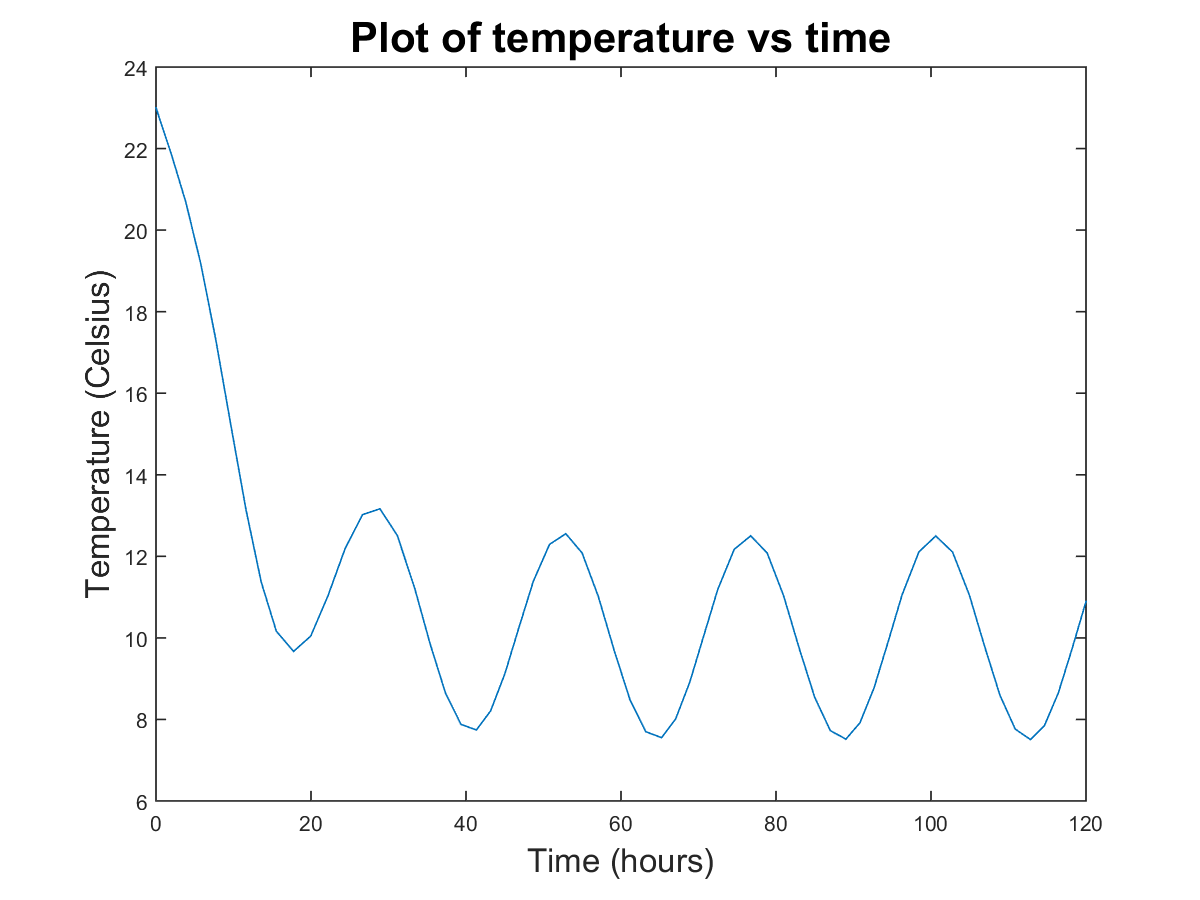
\includegraphics[width=3in]{graphics/Week08_Spring/W08GarageTemp_1}

The file 
  \href{http://www.mast.queensu.ca/~apsc171/MNTCP01/PracticeProblems/MATLAB/W08GarageTemp.m}{W08GarageTemp.m} 
has the MATLAB code that generated the graph above.

\item From the graph, it takes the building roughly 2 days (48 hours)
  to get into a repeating cycle of temperature variation.

\item Careful zooming of the graph (or a look at the $y$ values in the
  ode45 output) give a highest temperature of 12.5 (high) and 7.5
  (low), for a net fluctuation of approximately 2.6 degrees per day.

\item $k$ represents the coefficient of heat flow between the building
  and the environment. The bigger $k$ is, the {\em larger} the
  headflow between the two.  Since we're adding insulation, this
  should {\em reduce} the heat flow, and so {\em lower} the value of
  $k$.

\item A graph of the heat change over time, given better insulation,
  is shown below.

  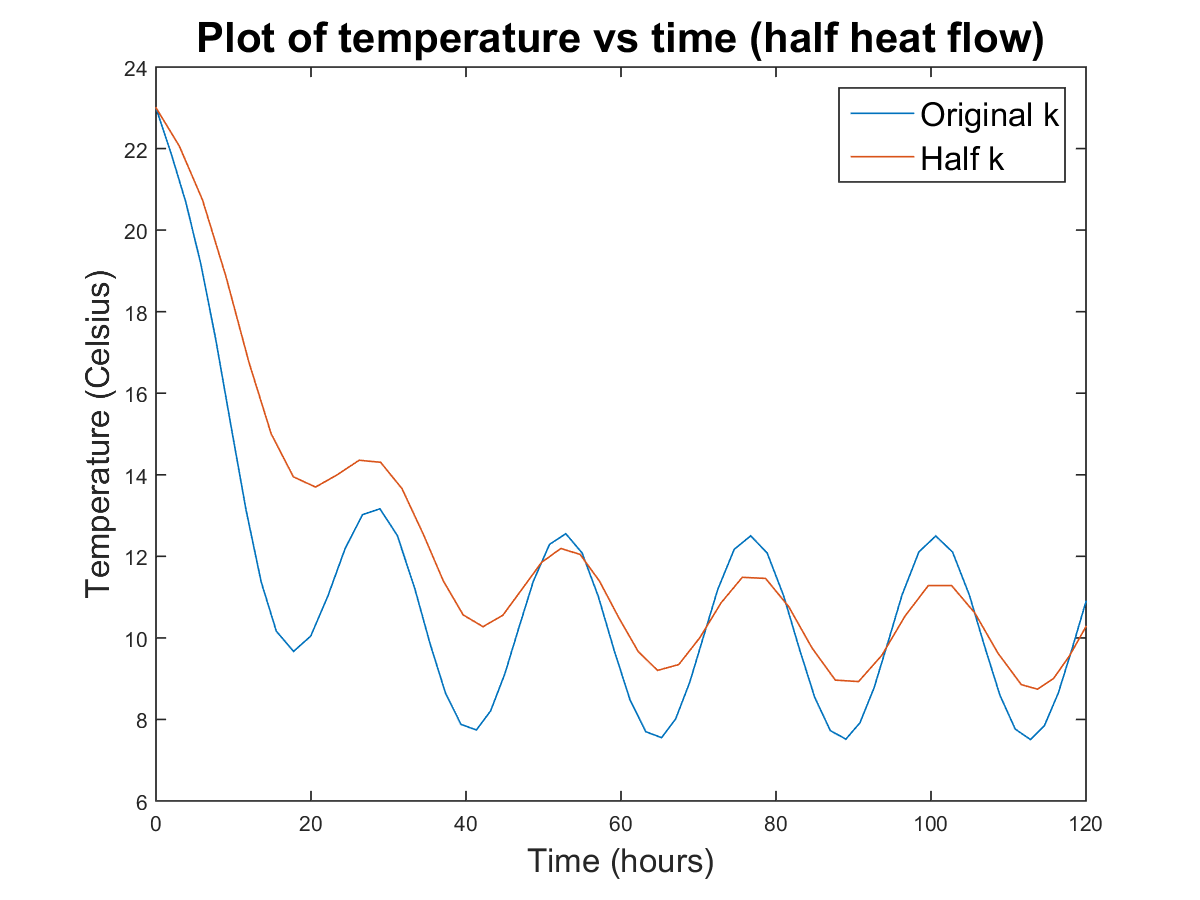
\includegraphics[width=3in]{graphics/Week08_Spring/W08GarageTemp_2}

\item Zooming in on the peaks of the {\bf red line} graph (new
  insulation model), the temperature now fluctuates between
  approximately 11.3 and 8.8 degrees Celsius, for a range of 2.5
  degrees.  This {\em is} roughly half the magnitude of the
  fluctuations we saw earlier.

\end{enumerate}
\end{Solution}


\hrulefill

\subsection*{Modelling Spring Systems}
% ******************************
\item  \label{SpringNoDampingNoFext}
  \begin{Question}
    \begin{minipage}[t]{0.6\linewidth}
\vspace{0pt}
Consider the single spring/mass system shown to the right, with no damper.

Newton's second law gives us the relationship:
\begin{align*}
ma & = \sum F = \Fspring \\
m x'' & = -k x 
\end{align*}
where $k$ is the spring constant.
    \end{minipage}
    \begin{minipage}[t]{0.3\linewidth}
\vspace{0pt}
\begin{center}
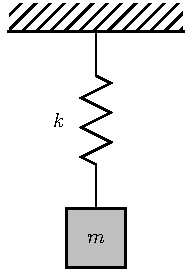
\includegraphics[width=1.0in]{graphics/Week08_Spring/SpringNoDamping}
\end{center}
    \end{minipage}


\begin{enumerate}
\item By hand, write this second order DE as a system of 1st order
  DEs, using the new variables $w_1 = x$ and $w_2 = x'$

\item Write a MATLAB function file called \verb#springDE1.m# starting
  with the first line \\
  \verb#function dw_dt = springDE1(t, w, m, k)# \\
  that implements the system of differential equations from part (a).
\item Write a MATLAB script that simulates the motion of the mass
  using $m = 0.5$ kg and $k = 10$ N/m.  Choose the time interval for
  the simulation so that 4-5 cycles of oscillation are shown.
\end{enumerate}
\end{Question}

\begin{Solution}
 \begin{enumerate}
 \item  The first-order system would be:
 \begin{align*}
 \frac{d}{dt} w_1 & = x' = w_2 \\
 \frac{d}{dt} w_2 & = x'' = \frac{1}{m} \left(-kx \right) = \frac{1}{m} \left(-k w_1  \right)
 \end{align*}

\item The function file  
  \href{http://www.mast.queensu.ca/~apsc171/MNTCP01/PracticeProblems/MATLAB/springDE1.m}{springDE1.m} 
  implements the differential equation system, with the $\Fext $ term
  left out.

\item The main script
\href{http://www.mast.queensu.ca/~apsc171/MNTCP01/PracticeProblems/MATLAB/W08SpringSimulation01.m}{W08SpringSimulation01.m} 
has the code that will run this simulation.

In the resulting plot, we see a very nice example of simple harmonic
motion.

\begin{center}
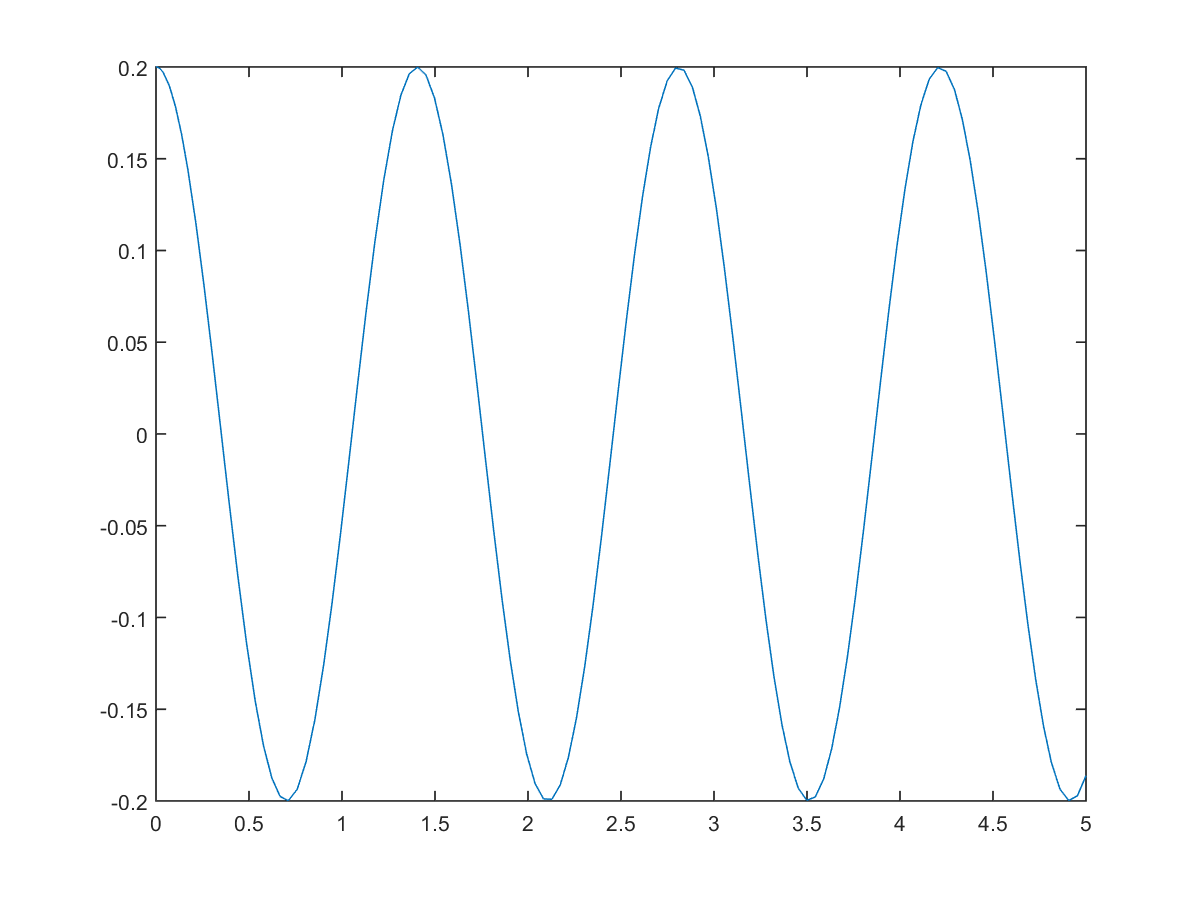
\includegraphics[width=3in]{graphics/Week08_Spring/W08SpringSimulation01}
\end{center}

\end{enumerate}
\end{Solution}



% ******************************
\item  \label{SpringNoDampingWithFext}
  \begin{Question}
    \begin{minipage}[t]{0.6\linewidth}
\vspace{0pt}
Consider the single spring/mass system shown to the right, with no damper.

This is the same as in Question \ref{SpringNoDampingNoFext}, except
with the addition of the $\Fext$ shown as an external applied force.

Newton's second law gives us the relationship:
\begin{align*}
ma & = \sum F = \Fspring + \Fext \\
m x'' & = -k x + \Fext 
\end{align*}
where $k$ is the spring constant.
    \end{minipage}
    \begin{minipage}[t]{0.3\linewidth}
\vspace{0pt}
\begin{center}
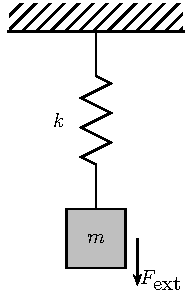
\includegraphics[width=1.0in]{graphics/Week08_Spring/SpringNoDampingWithFext}
\end{center}
    \end{minipage}


\begin{enumerate}
\item By hand, write this second order DE as a system of 1st order
  DEs, using the new variables $w_1 = x$ and $w_2 = x'$


\item We will now incorporate an external force of the form
  $F_{\mbox{ext}} = a \sin(b t)$. Write a MATLAB function file called
  \verb#springDE2.m# starting with the first line \\
  \verb#function dw_dt = springDE2(t, w, m, k, a, b)# \\
  that implements the system of differential equations from part (a).

\item Create a new MATLAB script.  In the script, set $m =0.5$ kg,
  $k = 10$ N/m, and use $a = 5$ and $b = 1$ in
  $F_{\mbox{ext}} = a \sin(bt)$.  Use \verb#ode45# to simulate the
  motion of the spring for 30 seconds (\verb#tspan = [0, 30]#), given
  an initial displacement of $x(0) = 0.2$ m, and initial velocity of
  zero: $x'(0) = 0$. \label{forced}

\item Explain why the motion looks so disorganized.

\item Repeat Question (\ref{forced}), but with an external force of
  $\Fext = \sin(4 t)$. Explain why the motion in this case has cyclic
  waves in its amplitude.


\end{enumerate}
  \end{Question}

\begin{Solution}
 \begin{enumerate}
 \item  The first-order system would be:
 \begin{align*}
 \frac{d}{dt} w_1 & = x' = w_2 \\
 \frac{d}{dt} w_2 & = x'' = \frac{1}{m} \left(-kx + \Fext\right) = \frac{1}{m} \left(-k w_1  + \Fext \right)
 \end{align*}

\item The file  
  \href{http://www.mast.queensu.ca/~apsc171/MNTCP01/PracticeProblems/MATLAB/springDE2.m}{springDE2.m} 
  implements the differential equation system, with new external force
  $\Fext = a \sin(bt)$.
\item The file 
\href{http://www.mast.queensu.ca/~apsc171/MNTCP01/PracticeProblems/MATLAB/W08SpringSimulation02.m}{W08SpringSimulation02.m} 
has the code that will run this simulation.

In the resulting plot, see some wildly varying and irregular
oscillations.

\begin{center}
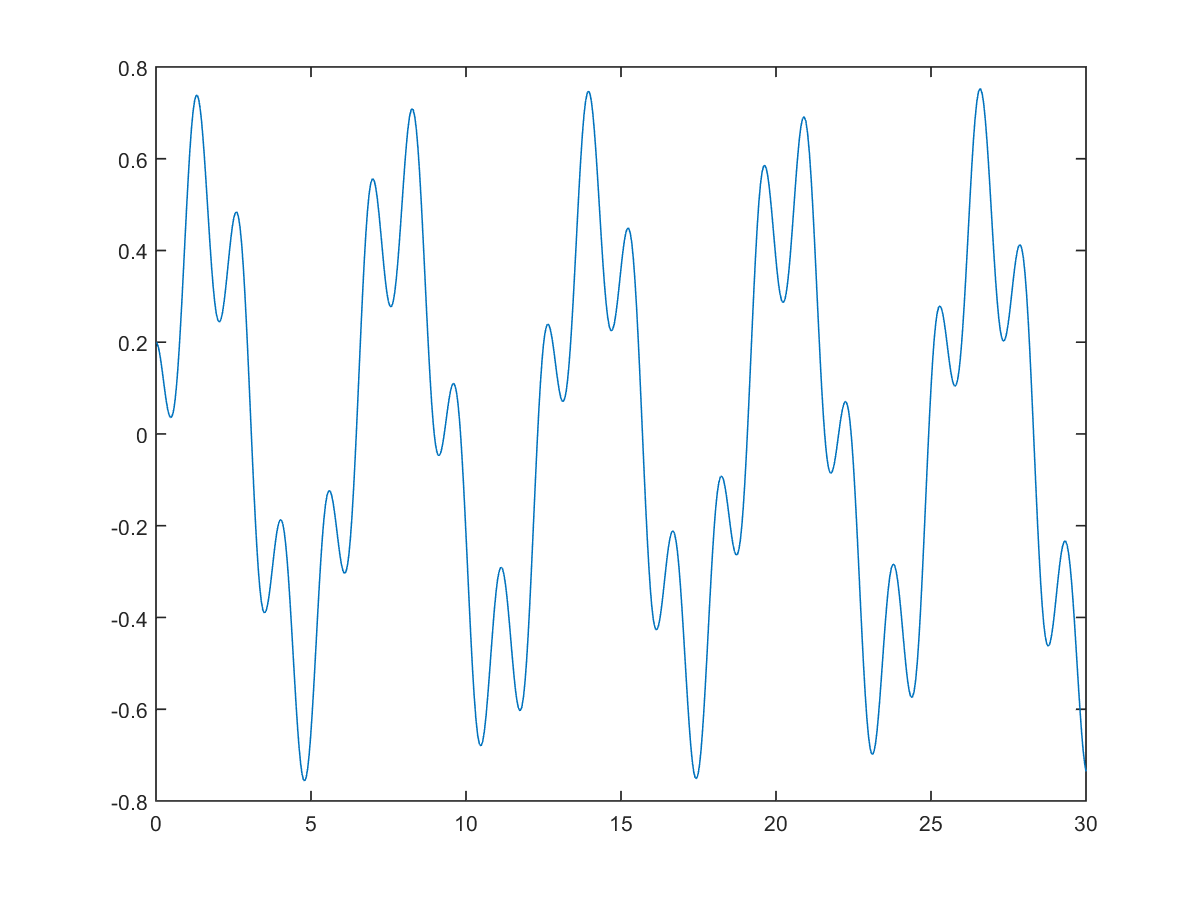
\includegraphics[width=3in]{graphics/Week08_Spring/W08SpringSimulation02}
\end{center}

\item The motion of the mass looks very disorganized because the
  natural frequency (the frequency at which the mass would oscillate
  if you just let swing on its own) is different from the frequency
  that we are pushing and pulling on it with through $\Fext$.

  Recall: the natural frequency of a spring/mass system is given by
  $\omega = \sqrt{k/m}$, which for this scenario gives $\omega = \sqrt{ \frac{25}{4}}$ 


\item 
The file 
  \href{http://www.mast.queensu.ca/~apsc171/MNTCP01/PracticeProblems/MATLAB/W08SpringSimulation02.m}{W08SpringSimulation02.m} 
  has the code that will run this simulation.  Here is a graph of the
  resulting mass motion.

\begin{center}
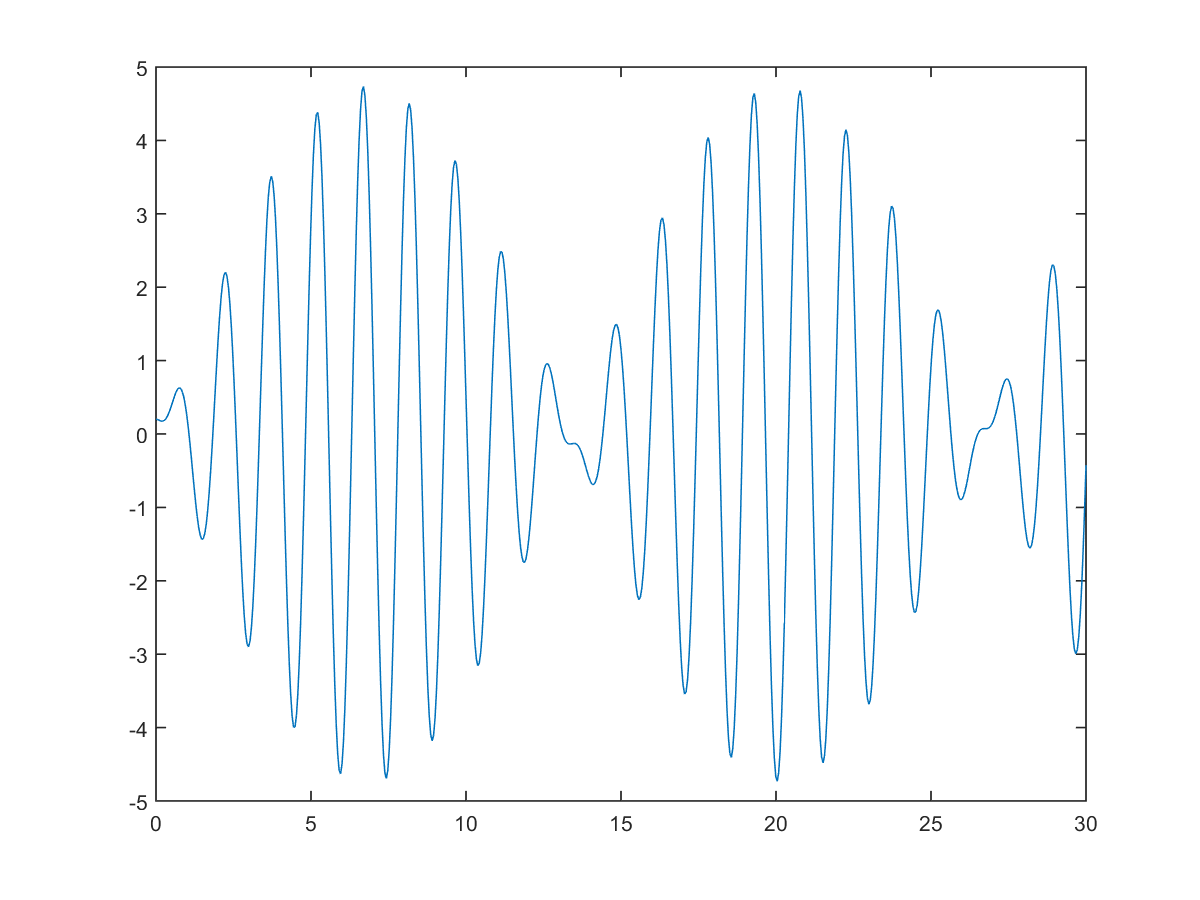
\includegraphics[width=3in]{graphics/Week08_Spring/W08SpringSimulation03}
\end{center}

In the plot, we see
  that the natural frequency and the regular stimulation by the
  outside force are close to each other: the natural frequency is
  $\omega = \sqrt{\frac{10}{0.5}} \approx 4.5$, rad/s, and the
  stimulating frequency is at $\omega = 4$ rad/s.  This close match of
  the frequencies leads to the phenonenon called {\em beats}, or {\em
    near resonance}.
\end{enumerate}
\end{Solution}

% ******************************
\item 
  \begin{Question}
    \begin{minipage}[t]{0.6\linewidth}
      \vspace{0pt} We return to the same single spring/mass system
      from Question \ref{SpringNoDampingWithFext}, shown to the right,
      with no damper.
      
The $\Fext$ shown is an external applied force.
    \end{minipage}
    \begin{minipage}[t]{0.3\linewidth}
\vspace{0pt}
\begin{center}
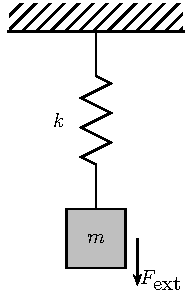
\includegraphics[width=1.0in]{graphics/Week08_Spring/SpringNoDampingWithFext}
\end{center}
    \end{minipage}


\begin{enumerate}
\item For a mass of $m = 5$ kg , and a spring constant of $k = 2$ N/m,
  what is the natural frequency of the system?
\item Define an external force of the form $\Fext = \sin(b t)$ that will
produce {\bf resonance} in the system.
\item Use MATLAB to simulate the motion of the spring, with your
  selected external force, using an initial condition where the mass
  starts at its equilibrium and at rest.
\item The system will break if the oscillations become too large,
  specifically if $x(t)$ exceeds 2 m (in the positive or negative
  directions).  Does the system break, and if so, how long does it
  take for the system to break?
\end{enumerate}
\end{Question}

\begin{Solution}
  \begin{enumerate}[(a)]
  \item The natural frequency of a spring/mass system is given by
    $\omega = \sqrt{\frac{k}{m}} = \sqrt{\frac{2}{5}} \approx 0.6325$
    rad/s.
  \item If we want to produce resonance in the oscillations, our
    applied force's frequency must be exactly at the same frequency as
    the natural frequency. That way, the natural oscillations and the
    applied force are perfectly synchronized, leading to a build-up of
    the energy in the system.  

    This means we should select $\Fext = sin( 0.6325 t)$.

  \item For this problem, we can recycle the differential equation
    code in
    \href{http://www.mast.queensu.ca/~apsc171/MNTCP01/PracticeProblems/MATLAB/springDE2.m}{springDE2.m}
    from Question \ref{SpringNoDampingWithFext}, because the forces
    (spring and $\Fext$) are in the same form as in that problem.

    In our new main script,
    \href{http://www.mast.queensu.ca/~apsc171/MNTCP01/PracticeProblems/MATLAB/W08Resonance1.m}{W08Resonance1.m}
    we will set up all the constants needed for the simulation:
    \begin{itemize}
    \item $m = 5$, $k = 2$, 
    \item $a = 1$ and $b= 0.6325$ to define
      $\Fext = a \sin(bt) = 1 \cdot \sin(0.6325 t)$.
    \end{itemize}

    Below is a graph of the simulated motion of the mass over 30
    seconds:
\begin{center}
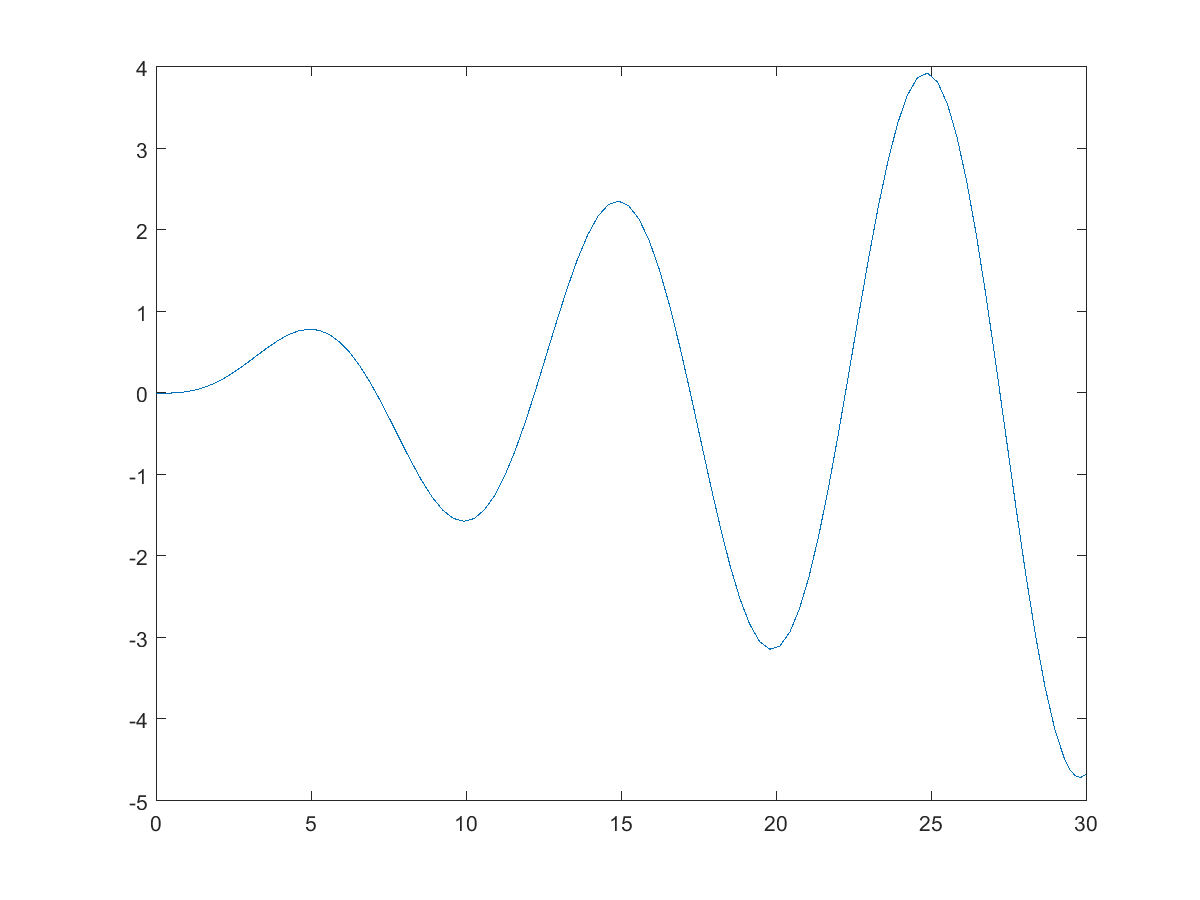
\includegraphics[width=0.4\linewidth]{graphics/Week08_Spring/W08SpringResonance1}
\end{center}

\item From the graph, we see that the amplitude of the oscillations
  are growing with every cycle, as expected when we induce resonance.  This means that the system {\em will } break at some point. 

  The specific limit we were given was that breakage will occur if
  $x(t)$ exceeds 2 m. Zooming in, we can see that the system will
  reach $x(t) \approx 2$ m around $t = 14$ seconds.

\begin{center}
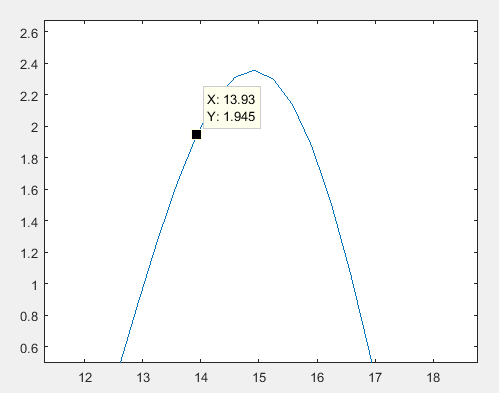
\includegraphics[width=0.4\linewidth]{graphics/Week08_Spring/W08Resonance1_BreakPoint}
\end{center}

  \end{enumerate}
\end{Solution}


% ******************************
\item 
  \begin{Question}
    \begin{minipage}[t]{0.6\linewidth}
      \vspace{0pt} Consider the damped system shown at right.

      The damping force exerted by the dashpot/damper is proportional
      to the velocity of the mass.

Newton's second law gives us the relationship:
\begin{align*}
ma & = \sum F = \Fspring + \Fdamping \\
m x'' & = -k x  - c x' 
\end{align*}
where $k$ is the spring constant in N/m, and $c$ is the damping
coefficient in N/(m/s).

    \end{minipage}
    \begin{minipage}[t]{0.3\linewidth}
\vspace{0pt}
\begin{center}
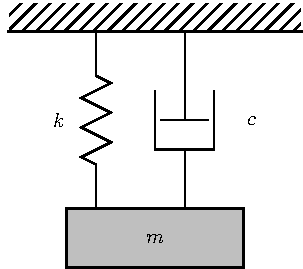
\includegraphics[width=0.9\linewidth]{graphics/Week08_Spring/W08DampedSpringNoFext}
\end{center}
    \end{minipage}

\begin{enumerate}[(a)]
\item By hand, write this second order DE as a system of 1st order
  DEs, using the new variables $w_1 = x$ and $w_2 = x'$

\item We define a system with a mass of $m = 10$ kg, spring constant
  $k = 2$ N/m, and a damping coefficient of $c = 0.4$ N/(m/s).  If the
  system is displaced by 0.5 m and then let go with zero initial
  velocity, use MATLAB to find out how long (in both seconds and
  cycles) it takes for the oscillations to reach approximately 10\% of
  their original amplitude.  Note: you will need to write both a
  MATLAB function for the differential equation, and a main script to
  run the simulation.
\item What damping coefficient would be needed for the oscillations to
  be reduced to 10\% of their original amplitude within 3 cycles?  You
  will need to estimate your answer based on guessing and checking
  against the graph.  Hint: add horizontal lines to the solution plot
  at $x = 0.05$ and $x = -0.05$ to see easily whether the oscillations
  are reduced to that level.
\end{enumerate}
\end{Question}

\begin{Solution}
  \begin{enumerate}[(a)]
 \item  The first-order system would be:
 \begin{align*}
 \frac{d}{dt} w_1 & = x' = w_2 \\
 \frac{d}{dt} w_2 & = x'' = \frac{1}{m} \left(-kx -c x'\right) = \frac{1}{m} \left(-k w_1  - c w_2\right)
 \end{align*}

\item To simulate the motion of the spring/mass system, we need a
  function file with the differential equation, which we called
  \href{http://www.mast.queensu.ca/~apsc171/MNTCP01/PracticeProblems/MATLAB/springDEDamped.m}{springDEDamped.m},
  and a main script, which we called
  \href{http://www.mast.queensu.ca/~apsc171/MNTCP01/PracticeProblems/MATLAB/W08DampedSpringSystem.m}{W08DampedSpringSystem.m}.

  Here is the graph of the resulting motion, showing a nice
  oscillatory pattern, but the amplitude diminishing over time due to
  the damping.

\begin{center}
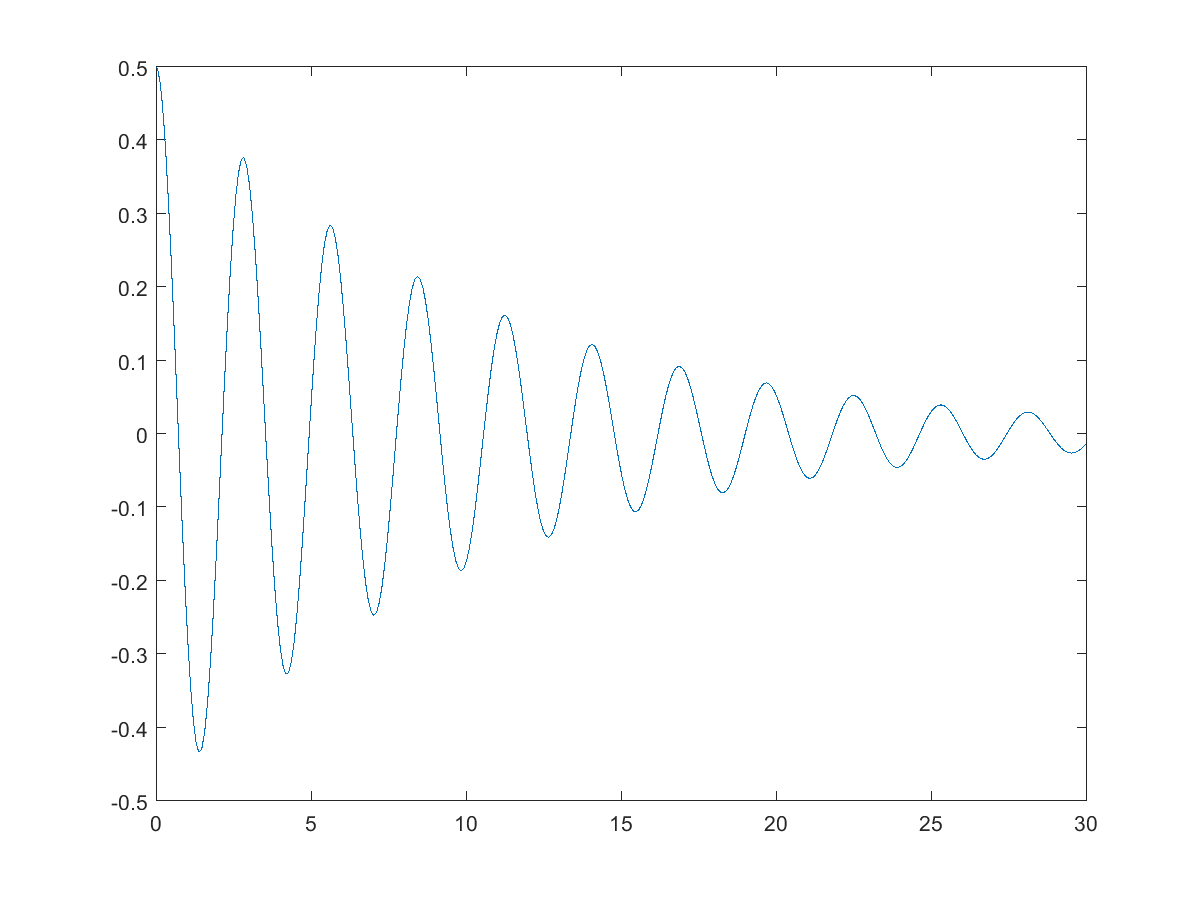
\includegraphics[width=3in]{graphics/Week08_Spring/W08DampedSpring1A}
\end{center}


seconds, or between 8 and 9 cycles.

\begin{center}
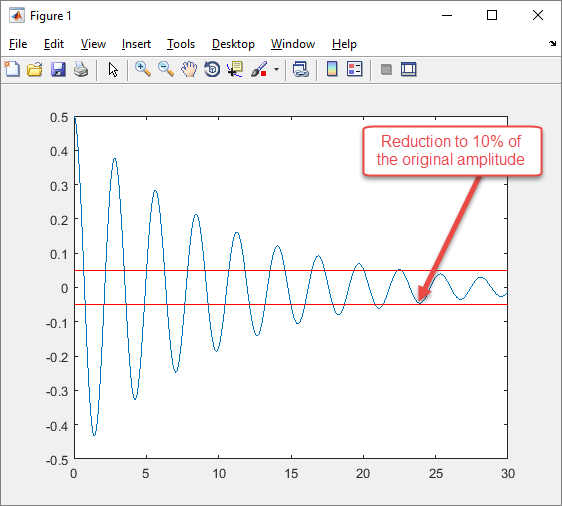
\includegraphics[width=3in]{graphics/Week08_Spring/W08DampedSpring1B}
\end{center}

\item Using $c = 1.1$ N/(m/s) gives the required damping, putting the amplitude
of the oscillations below 10\% of their original magnitude after 3 cycles.

\begin{center}
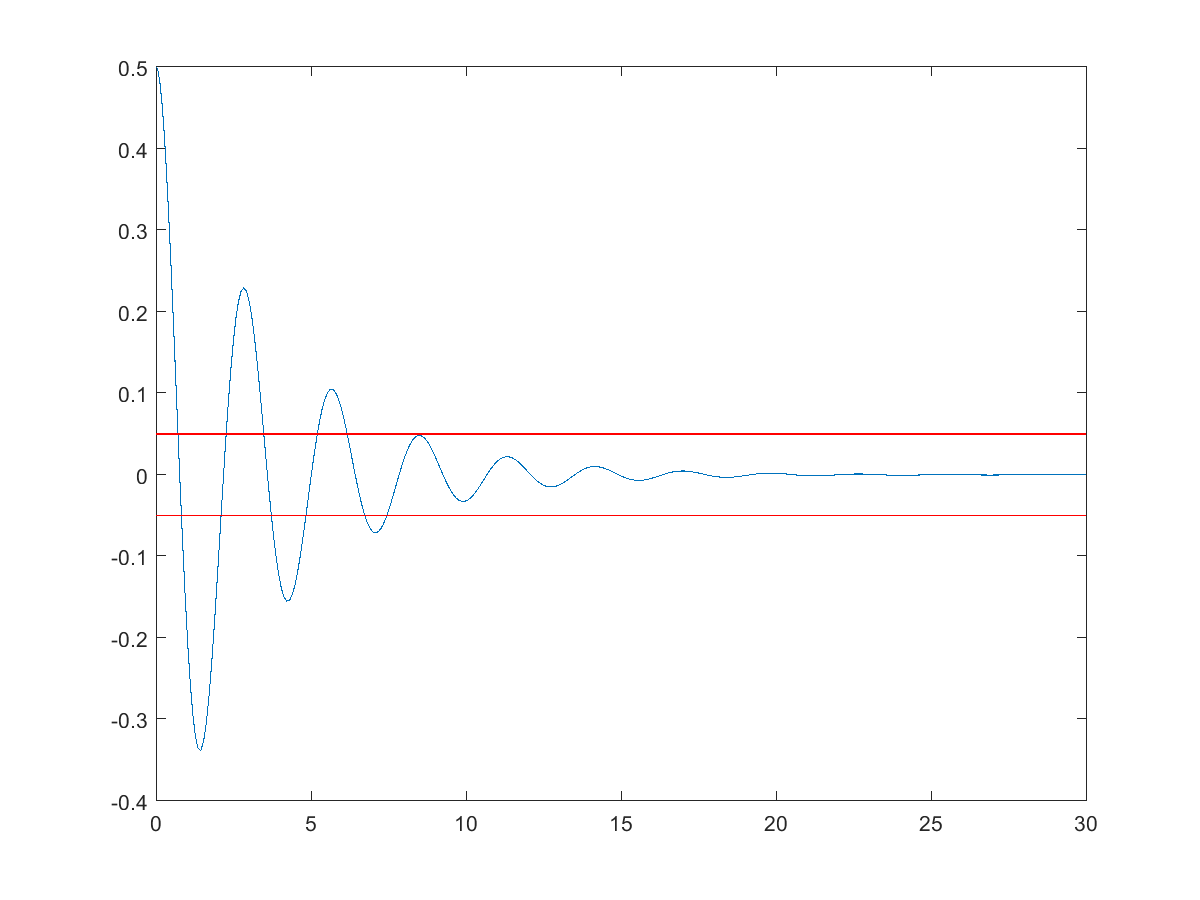
\includegraphics[width=3in]{graphics/Week08_Spring/W08DampedSpring1C}
\end{center}

 

  \end{enumerate}
\end{Solution}


% %****************
\item 
\begin{Question}
  For a spring/mass system with $m=1$ kg, $c=0.5$ N/(m/s), and $k=45$,
  approximately what frequency of external forcing would produce the
  largest amplitude steady-state vibration?  Give your answer to the
  nearest 0.5 rad/s.

  You will need to estimate the answer based on guessing and checking
  against the graph.
 \end{Question}

 \begin{Solution}
   The natural frequency is going to be near
   $\omega = \sqrt{k/m} \approx 6.7$ rad/s.

   To run the simulation in MATLAB, we know we need to build the
   differential equation based on the sum of the forces in MATLAB.  $ma = \sum F$ gives us
$$ m x'' = -kx - c x' + \sin(bt)$$
where $b$ is the frequency we can experiment with to maximize the
steady-state oscillations.

The first-order system version of this is: 
 \begin{align*}
 \frac{d}{dt} w_1 & = x' = w_2 \\
 \frac{d}{dt} w_2 & = x'' =  \frac{1}{m} \left(-kx -c x'+ \sin(bt) \right) \\
& = \frac{1}{m} \left(-k w_1  - c w_2 + \sin(bt) \right)
 \end{align*}

 We built this system of differential equations into the file
 \href{http://www.mast.queensu.ca/~apsc171/MNTCP01/PracticeProblems/MATLAB/springDEDampedAndForced.m}{springDEDampedAndForced.m} 
and the main script
 \href{http://www.mast.queensu.ca/~apsc171/MNTCP01/PracticeProblems/MATLAB/W08DampedSpringSystem3.m}{W08DampedSpringSystem3.m} 

 If we are only interested in the steady-state behaviour, then the
 initial conditions won't matter (their influence fades in the long
 run). We make the easiest choice, which is the mass starting at
 equilibrium at rest, $x(0) = 0$ and $x'(0) = 0$.

 Below is a graph showing the response of the system to
 $b = 5, 5.5, 6, 6.5$ and 7 rad/s, and then the graph for $b = 6.5$
 rad/s only.

\begin{center}
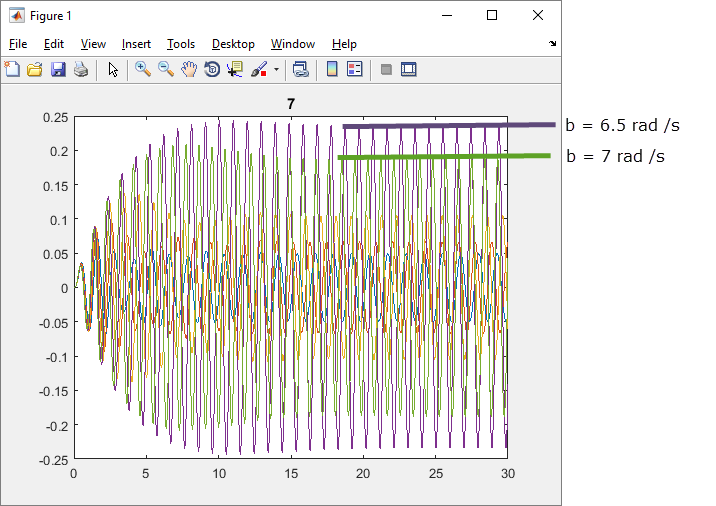
\includegraphics[height=2.6in]{graphics/Week08_Spring/W08DampedAndForced1}
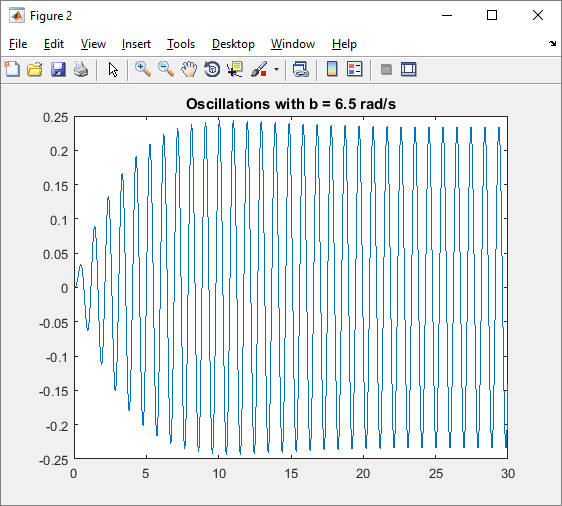
\includegraphics[height=2.6in]{graphics/Week08_Spring/W08DampedAndForced2}
\end{center}

Looking for the steady-state oscillations means looking at the
amplitudes once the graph steadies into a regular repeating pattern.
The graph corresponding to $\Fext = \sin(6.5~t)$ is the graph with the
highest amplitude once that steady-state oscillation pattern is
reached.


 \end{Solution}

\end{enumerate}





\end{document}
